%%%%%%%%%%%%%%%%%%%%%%%%%%%%%%%%%%%%%%%%%%%%%%%%%%%%%%%%%%%%%%%%%%%%%%
\begin{frame}[fragile]\frametitle{}
\begin{center}
{\Large Arrays and Lists}
\end{center}

\end{frame}

%%%%%%%%%%%%%%%%%%%%%%%%%%%%%%%%%%%%%%%%%%%%%%%%%%%%%%%%%%%%%%%%%%%%%%
\begin{frame}
	\frametitle{Why study the list?}
		What do we use lists for?	

		\begin{itemize}
			\item To store a collection of data.
			\item To build other more complex/refined data structures!
		\end{itemize}
\end{frame}

%%%%%%%%%%%%%%%%%%%%%%%%%%%%%%%%%%%%%%%%%%%%%%%%%%%%%%%%%%%%%%%%%%%%%%
\begin{frame}
	\frametitle{Lists in Python}
		How do lists in Python work?

		\begin{itemize}
			\item 		They are array-based!
			\item   	So what's an array then?
	\end{itemize}
\end{frame}

%%%%%%%%%%%%%%%%%%%%%%%%%%%%%%%%%%%%%%%%%%%%%%%%%%%%%%%%%%%%%%%%%%%%%%
\begin{frame}
	\frametitle{Arrays}
	\begin{block}{Array}
		An array is a block of memory of fixed size that can hold multiple items of data.
	\end{block}	


	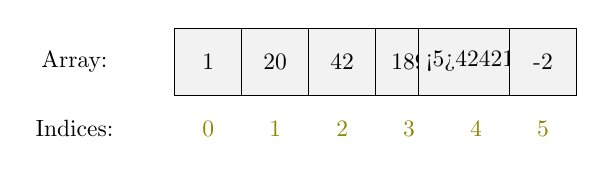
\begin{tikzpicture}[scale=0.85, transform shape]
	\foreach \x/\val in {0/1,1/20,2/42,3/189,4/\alt<5>{\alert{4242}}{17},5/-2}{
	\node[draw,rectangle, fill=gray!10, minimum size =1cm] (c) at (\x,0) {\val};
	\node[olive] (index) at (\x,-1) {\x};
}
\node[] at (-2,0) {Array:};
\node[] at (-2,-1) {Indices:};
\end{tikzpicture}


			\begin{itemize}
			\item 	\lstinputlisting{src/array.py}
			\item
			\item 	\lstinputlisting{src/array2.py}
			\item
			\item 	\lstinputlisting{src/array3.py}
	\end{itemize}


\end{frame}

%%%%%%%%%%%%%%%%%%%%%%%%%%%%%%%%%%%%%%%%%%%%%%%%%%%%%%%%%%%%%%%%%%%%%%
\begin{frame}
	\frametitle{Arrays}

	
			How does this differ from a list?

			\begin{itemize}
				\item It's just memory, no things like \texttt{a.sort()}.
				\item It is \textit{finite}!
			\end{itemize}

\end{frame}

%%%%%%%%%%%%%%%%%%%%%%%%%%%%%%%%%%%%%%%%%%%%%%%%%%%%%%%%%%%%%%%%%%%%%%
\begin{frame}
	\frametitle{Array-based lists}

		An array-based list (like the \texttt{list} in Python) uses an array internally.

		How can we then grow the list (seemingly) infinitely?
		\begin{enumerate}[A.]
			\item The list uses multiple arrays stitched together.
			\item The list also has a finite size from the start, we just never notice.
			\item The list creates a new array of size $n+1$ when the array if full.
			\item The list creates a new array of size $n*2$ when the array if full.
			\item I don't know.
		\end{enumerate}

\end{frame}

%%%%%%%%%%%%%%%%%%%%%%%%%%%%%%%%%%%%%%%%%%%%%%%%%%%%%%%%%%%%%%%%%%%%%%
\begin{frame}
	\frametitle{Stitching arrays together}
		The list uses multiple arrays stitched together.
		\begin{itemize}
			\item Although technically possible, keeping track of all of it is hell not pleasant.
			\item There are also benefits to having one continuous block of memory.
				\begin{itemize}
					\item For instance spacial caching benefits (Google it, if you are intrigued ;))
				\end{itemize}
				
			\item But the idea isn't a bad one per se. Having only single items blocks, forms the basis of the list we study
				after the break!
		\end{itemize}
\end{frame}

%%%%%%%%%%%%%%%%%%%%%%%%%%%%%%%%%%%%%%%%%%%%%%%%%%%%%%%%%%%%%%%%%%%%%%
\begin{frame}
	\frametitle{A hidden maximum size?}
		The list also has a finite size from the start, we just never notice.
		\begin{itemize}
			\item Nope, we can grow it so long as there is memory available.
		\end{itemize}
\end{frame}

%%%%%%%%%%%%%%%%%%%%%%%%%%%%%%%%%%%%%%%%%%%%%%%%%%%%%%%%%%%%%%%%%%%%%%
\begin{frame}
	\frametitle{So... New arrays then?}
		When the initial array is full, we create a new one with more capacity.\\
		We copy over all existing elements into the new array\dots\\
		And we now have new space to grow!
	
		But by how much should we grow?	
	
	Observations:
		\begin{itemize}
			\item Adding one item, can trigger a full copy of the array...
			\item Does that make \texttt{append} an $O(n)$ operation?
		\end{itemize}
\end{frame}

%%%%%%%%%%%%%%%%%%%%%%%%%%%%%%%%%%%%%%%%%%%%%%%%%%%%%%%%%%%%%%%%%%%%%%
\begin{frame}
	\frametitle{Just enough room}
		The list creates a new array of size $n+1$ when the array if full.
		
		Doing it often.
	
		What happens when we add $n$ elements to a list of size $1$?
		
		\begin{itemize}
			\item Every time we need to copy the full list.
			\item So $O(\sum\limits_{i=1}^{n}i)$ time in total.
			\item So $O(n^2)$ to add $n$ elements\dots
		\end{itemize}
\end{frame}

%%%%%%%%%%%%%%%%%%%%%%%%%%%%%%%%%%%%%%%%%%%%%%%%%%%%%%%%%%%%%%%%%%%%%%
\begin{frame}
	\frametitle{More than enough room}
		The list creates a new array of size $n*2$ when the array if full.
		
		Doing it often
	
		What happens when we add $n$ elements?
\end{frame}

%%%%%%%%%%%%%%%%%%%%%%%%%%%%%%%%%%%%%%%%%%%%%%%%%%%%%%%%%%%%%%%%%%%%%%
\begin{frame}
	\frametitle{Amortised run time}
		Some operations have varying run times, but can be shown to be efficient when repeated multiple times. We call
		this an amortised run time.
	
Consider \ldots
		\begin{itemize}
			\item Consider a list of size $1$ and we add $n$ elements to it.
			\item This means we double the size of the list $\log_2(n)$ times.
			\item This means that in total we have: $O(n)$ time to add all elements.
			\item And $O\left(\sum\limits_{i=1}^{\log_2(n)} 2^i\right)$ operations to copy when the list grows.
			\item This geometric sequence gets us to: $O(2^{\log_2(n)}) = O(n)$ operations.
			\item So $O(n)$ to add $n$ items!
		\end{itemize}
		
		We call this an amortised run time of $O(1)$ for the append operation!
\end{frame}

%%%%%%%%%%%%%%%%%%%%%%%%%%%%%%%%%%%%%%%%%%%%%%%%%%%%%%%%%%%%%%%%%%%%%%
\begin{frame}
	\frametitle{Inserting}
	\begin{columns}
		\column{0.455\textwidth}

		\begin{block}{Let's insert}
			What is the time complexity of \texttt{l.insert(index,value)} when \texttt{len(l)}=n?
			\begin{enumerate}[A.]
				\item $O(1)$
				\item $O(\textit{index})$
				\item $O(n - \textit{index})$
				\item $O(n)$
				\item $O(n^2)$
				\item I don't know.
			\end{enumerate}
		\end{block}
		
		\column{0.455\textwidth}
		\begin{block}{Let's insert}
			We need to shift all elements after \texttt{index}, so $O(n-\textit{index})$
		\end{block}
		
		\begin{block}{Inserting at the front}
			This means prepending is $O(n)$ for array-based lists!
		\end{block}	
	\end{columns}
\end{frame}

%%%%%%%%%%%%%%%%%%%%%%%%%%%%%%%%%%%%%%%%%%%%%%%%%%%%%%%%%%%%%%%%%%%%%%
\begin{frame}
	\frametitle{Removing an item}
	\begin{columns}
		\column{0.455\textwidth}
		\begin{block}{Let's pop}
			What is the time complexity of \texttt{l.pop(index)} when \texttt{len(l)}=n?
			\begin{enumerate}[A.]
				\item $O(1)$
				\item $O(\textit{index})$
				\item $O(n - \textit{index})$
				\item $O(n)$
				\item $O(n^2)$
				\item I don't know.
			\end{enumerate}
		\end{block}
		
		\column{0.455\textwidth}
		\begin{block}{Let's pop}
			We need to shift all elements after \texttt{index}, so $O(n-\textit{index})$.
		\end{block}
		
		\begin{block}{Inserting at the front}
			This means removing the first item is $O(n)$ for array-based lists!
		\end{block}	
	\end{columns}
\end{frame}

%%%%%%%%%%%%%%%%%%%%%%%%%%%%%%%%%%%%%%%%%%%%%%%%%%%%%%%%%%%%%%%%%%%%%%
\begin{frame}
	\frametitle{Removing an item}
	\begin{columns}
		\column{0.455\textwidth}
		\begin{block}{Let's remove}
			What is the time complexity of \texttt{l.remove(value)} when \texttt{len(l)}=n?
			\begin{enumerate}[A.]
				\item $O(1)$
				\item $O(\textit{index})$, where index is the index of the value.
				\item $O(n - \textit{index})$, where index is the index of the value.
				\item $O(n)$
				\item $O(n^2)$
				\item I don't know.
			\end{enumerate}
		\end{block}
		
		\column{0.455\textwidth}
		\begin{block}{Let's remove}
			We need to find the element so $O(\textit{index})$.\\
			We need to shift all elements after \texttt{index}, so $O(n-\textit{index})$.\\
			Together this is $O(n)$.
		\end{block}
	\end{columns}
\end{frame}

%%%%%%%%%%%%%%%%%%%%%%%%%%%%%%%%%%%%%%%%%%%%%%%%%%%%%%%%%%%%%%%%%%%%%%
\begin{frame}
	\frametitle{Freeing up memory}
	\begin{block}{Freeing up space}
		When we remove sufficient items, we can free up space again.\\
		We do this when 25\% of the capacity is used.
	\end{block}	
	
	\begin{block}{Why 25\%?}
		Why not just when we drop below 50\% again?
	\end{block}
	
	\begin{block}{Thrashing}
		Thrashing is repeatedly claiming and releasing memory (and in this case copying the array).\\
		To avoid this, we use a different bound on when we release memory.
	\end{block}
\end{frame}

%%%%%%%%%%%%%%%%%%%%%%%%%%%%%%%%%%%%%%%%%%%%%%%%%%%%%%%%%%%%%%%%%%%%%%
\begin{frame}
	\frametitle{Lists in Python}
	So to summarise:
	\begin{itemize}
		\item Insert first element: $O(n)$.
		\item Insert at index $k$: $O(n-k)$.
		\item Append: amortised $O(1)$.
		\item Remove first element: $O(n)$.
		\item Remove last element: amortised $O(1)$.
		\item Remove index $k$: $O(n-k)$.
		\item Search (discussed last week): $O(n)$.
	\end{itemize}
\end{frame}

%%%%%%%%%%%%%%%%%%%%%%%%%%%%%%%%%%%%%%%%%%%%%%%%%%%%%%%%%%%%%%%%%%%%%%
\begin{frame}[fragile]\frametitle{}
\begin{center}
{\Large Linked Lists}
\end{center}

\end{frame}

%%%%%%%%%%%%%%%%%%%%%%%%%%%%%%%%%%%%%%%%%%%%%%%%%%%%%%%%%%%%%%%%%%%%%%
\begin{frame}
	\frametitle{What do we want to solve?}
	
		Two things in the array-based implementation that we hope to solve:
		\begin{enumerate}
			\item Only use space for items we actually use.
			\item Allow for efficient ($O(1)$?) adding and removing at the front of the list.
		\end{enumerate}
	
		Why do we want this efficient adding/removing?
\end{frame}

%%%%%%%%%%%%%%%%%%%%%%%%%%%%%%%%%%%%%%%%%%%%%%%%%%%%%%%%%%%%%%%%%%%%%%
\begin{frame}
	\frametitle{The notion of a linked list}
	% \begin{columns}
		% \column{0.455\textwidth}
			\begin{itemize}
				\item We build a list of blocks, starting with one item/block (we call this the \alert{head})
				\item We can then add another.
				\item These are connected, we can go from the first to the second item.
				\item So let's add one more item.
				\item We should also indicate when we have reached the end (we call this the \alert{tail}).
			\end{itemize}
		% \column{0.455\textwidth}
		% % Tikz template taken from: https://tex.stackexchange.com/a/19288
\begin{tikzpicture}[list/.style={draw}]

  \node[list] (A) {42};
	\only<2->{
  \node[list] (B) {99};
}
	\only<3->{
  \draw[] let \p1 = (A.two), \p2 = (A.center) in (\x1,\y2) -- (B);
}
	\only<4->{
  \node[list] (C) {12};
  \draw[] let \p1 = (B.two), \p2 = (B.center) in (\x1,\y2) -- (C);
}
\only<5->{
  \node[draw,inner sep=6pt] (D) {};
  \draw (D.north east) -- (D.south west);
  \draw (D.north west) -- (D.south east);
  \draw[] let \p1 = (C.two), \p2 = (C.center) in (\x1,\y2) -- (D);
}
\end{tikzpicture}	

	% \end{columns}
\end{frame}

%%%%%%%%%%%%%%%%%%%%%%%%%%%%%%%%%%%%%%%%%%%%%%%%%%%%%%%%%%%%%%%%%%%%%%
\begin{frame}
	\frametitle{How does this work now?}
	\framesubtitle{Searching for an item}	
	The approach:
	\begin{enumerate}
		\item Start at the head of the list.
		\item If this is is the item we need, return True.
		\item Else if this is the tail, return False.
		\item Else, move to the next item of the list and go to step 2.
	\end{enumerate}

	% % Tikz template taken from: https://tex.stackexchange.com/a/19288
\begin{tikzpicture}[list/.style={draw}]

	\node[list,on chain,onslide=<1-2>{red}] (A) {42};
	\node[list,on chain,onslide=<3>{red}] (B) {99};
  \draw[] let \p1 = (A.two), \p2 = (A.center) in (\x1,\y2) -- (B);
  \node[list,on chain,onslide=<4>{red}] (C) {12};
  \draw[] let \p1 = (B.two), \p2 = (B.center) in (\x1,\y2) -- (C);
	\node[on chain,draw,inner sep=6pt,onslide=<5>{red}] (D) {};
	\draw[onslide=<5>{red}] (D.north east) -- (D.south west);
	\draw[onslide=<5>{red}] (D.north west) -- (D.south east);
  \draw[] let \p1 = (C.two), \p2 = (C.center) in (\x1,\y2) -- (D);
\end{tikzpicture}	

	

	\lstinputlisting{src/ll_search.py}

\end{frame}

%%%%%%%%%%%%%%%%%%%%%%%%%%%%%%%%%%%%%%%%%%%%%%%%%%%%%%%%%%%%%%%%%%%%%%
\begin{frame}
	\frametitle{Getting an item!?}
	\framesubtitle{Getting item at index $i$}

	\begin{itemize}
		\item There is no easy way to access the $i$th item other than to `walk' there.
		\item So $O(\textit{index})$ to get the item at a certain \texttt{index}.
	\end{itemize}
	\lstinputlisting{src/ll_get.py}
\end{frame}

%%%%%%%%%%%%%%%%%%%%%%%%%%%%%%%%%%%%%%%%%%%%%%%%%%%%%%%%%%%%%%%%%%%%%%
\begin{frame}
	\frametitle{Inserting at the head or tail}
	\begin{itemize}
		\item Take the current head or tail.
		\item And put the new node before or after it :)
		\item \alert{$O(1)$ time!}
	\end{itemize}	


\end{frame}

%%%%%%%%%%%%%%%%%%%%%%%%%%%%%%%%%%%%%%%%%%%%%%%%%%%%%%%%%%%%%%%%%%%%%%
\begin{frame}
	\frametitle{Inserting at the head or tail}

	
	\begin{itemize}
		\item \lstinputlisting{src/ll_prepend.py}
		
		\item 
				
		\item \lstinputlisting{src/ll_append.py}
	\end{itemize}	

\end{frame}

%%%%%%%%%%%%%%%%%%%%%%%%%%%%%%%%%%%%%%%%%%%%%%%%%%%%%%%%%%%%%%%%%%%%%%
\begin{frame}
	\frametitle{Assumptions, Unfortunately}
	\begin{itemize}
		\item To do \texttt{add\_last} in constant time, we need a reference to the \texttt{tail}.
		\item Many implementations of Singly-Linked Lists do not have this.
		\item What do I mean with `Singly' Linked List?	
		\item Well, it's not doubly linked
		\item In other implementations, we can both go forwards and backwards!	
	\end{itemize}	

\end{frame}

%%%%%%%%%%%%%%%%%%%%%%%%%%%%%%%%%%%%%%%%%%%%%%%%%%%%%%%%%%%%%%%%%%%%%%
\begin{frame}
	\frametitle{Doubly-Linked Lists}
	\begin{itemize}
		\item A singly linked list: 	Only has connections in one direction.	
		\item A doubly linked list: 	Has connections in both directions.
	\end{itemize}	

\end{frame}

%%%%%%%%%%%%%%%%%%%%%%%%%%%%%%%%%%%%%%%%%%%%%%%%%%%%%%%%%%%%%%%%%%%%%%
\begin{frame}
	\frametitle{Inserting an item}
	\framesubtitle{What to do?}
	\begin{columns}
		\column{0.255\textwidth}
	\begin{itemize}
		\item Navigate to the place where we want to insert the item ($O(\textit{index})$)
			
		\item Add the item: $O(1)$
			
		\item So $O(\textit{index})$ time!
	\end{itemize}
			
		\column{0.755\textwidth}
		
	\lstinputlisting{src/ll_insert.py}
			
	\end{columns}
\end{frame}

%%%%%%%%%%%%%%%%%%%%%%%%%%%%%%%%%%%%%%%%%%%%%%%%%%%%%%%%%%%%%%%%%%%%%%
\begin{frame}
	\frametitle{Removing an item}

		What is the time complexity of removing the first and last item in a singly linked list?

		\begin{enumerate}[A.]
			\item $O(1)$ for the first, $O(1)$ for the last.
			\item $O(1)$ for the first, $O(n)$ for the last.
			\item $O(n)$ for the first, $O(1)$ for the last.
			\item $O(n)$ for the first, $O(n)$ for the last.
			\item I don't know.
		\end{enumerate}


\end{frame}

%%%%%%%%%%%%%%%%%%%%%%%%%%%%%%%%%%%%%%%%%%%%%%%%%%%%%%%%%%%%%%%%%%%%%%
\begin{frame}
	\frametitle{Removing an item}


		\begin{itemize}
			\item $O(1)$ time.
			
			\item \lstinputlisting{src/ll_remove_first.py}

		\item 
		
			\item $O(n)$ time.

			\item \lstinputlisting{src/ll_remove_last.py}
	\end{itemize}

\end{frame}

%%%%%%%%%%%%%%%%%%%%%%%%%%%%%%%%%%%%%%%%%%%%%%%%%%%%%%%%%%%%%%%%%%%%%%
\begin{frame}
	\frametitle{Improvements!}
	
			Note that in a doubly-linked list we can remove the last item in $O(1)$ time!
			
			We can just use \texttt{tail.prev} to find the last-but-one element in constant time!
			
\end{frame}

%%%%%%%%%%%%%%%%%%%%%%%%%%%%%%%%%%%%%%%%%%%%%%%%%%%%%%%%%%%%%%%%%%%%%%
\begin{frame}
	\frametitle{So to summarise}

	\begin{tabular}{l | c | c | c}
	Operation & Array-based list & SLL & DLL \\	
	\midrule
	Get element $k$ & $O(1)$ &$O(k)$ & $O(k)$ \\
	
	Insert first element& $O(n)$ & $O(1)$ & $O(1)$\\
	Insert at index $k$& $O(n-k)$ & $O(k)$ & $O(\min(k,n-k))$\\
	Append (amortised)& $O(1)$ & $O(1)$ & $O(1)$\\
	
	Remove first element& $O(n)$ & $O(1)$ & $O(1)$\\
	Remove last element& $O(1)$ & $O(n)$ & $O(1)$\\
	Remove index $k$& $O(n-k)$ & $O(k)$ & $O(\min(k,n-k))$\\
	
	Search & $O(n)$ & $O(n)$ & $O(n)$\\
	\end{tabular}


\end{frame}

